\chapter{Implementation}

	\section{Infrastructure}
		
		\subsubsection{Team management}
		
			Considering the kind of event bounded to the game usage is clear that the team registration must be done long \emph{before} the event.
			
			For this, a simple website needs to be developed, where teams must be able to enrol for events, specifying the emails of all team members and a reference person which will take care of the team management (e.g., player removal or substitution).
			In this way organizers will be able to directly communicate with all players of a given event.
			This project won't cover that part and focus only on the mobile application part.
		
		\subsubsection{Data storage and manipulation}
			
			The data management is achieved using a new cloud platform, Firebase, instead of relying on an old-style SQL database accessed from a PHP/Java environment.
			This service does a great job keeping data in sync between heterogeneous devices and offers a powerful API together with a solid yet flexible security system based on data access rules.
			One drawback is that complex queries cannot be performed with a single request and must be done using nested calls to the database even if the heavy optimization mitigates this problem.
		
		\subsubsection{Game}
		
			Being backed by Firebase, the first idea was to avoid the back-end server, implementing some sort of all-in-app distributed game logic.
			Unluckily, it resulted obvious that game status and phases, together with some conditions checks, needed a centralized code to be managed easily.
			Actually this constraint is more a design-driven choice than a mandatory one: all the game logic \emph{can} be realized directly on the mobile application, synchronizing between all devices, but this results in messy code and opens some security issues: not the most desirable scenario at all.
			Considering this, the KISS (Keep It Simple, Stupid) approach had been followed and the two aspects of the game were separated.
			
			\newpage
			
			\paragraph{Game logic}
			
				To support the game logic, a Java task on the server will run in loop interacting with the real-time database observing the actions made by the players and eventually acting on his own to change the game internal status. In particular, it takes care of:
				\begin{itemize}
					\item \textbf{initialization:} preparatory steps to execute before a match takes place (initial status, board set-up);
					\item \textbf{phases:} manages phase changes and the timers associated with them;
					\item \textbf{objectives:} check every turn if a team reached its objective;
					\item \textbf{events:} manages the chances of an event to take place,  random selection between the available ones and the application of its effects;
					\item \textbf{status reset:} every temporary status change (zones power-ups and events effects) is reset to its original value at the end of turn;
					\item \textbf{power-up:} applies effects of the power-ups;
					\item \textbf{log:} record all match actions and events to enable post-match studies and replays.  
				\end{itemize}
				
				The timers that the game logic must share with the application are saved on the database as their expiration date. In this way it is possible to every device in any moment to calculate the missing time to the expiration and set an internal time-out on their own.
			
			\paragraph{Players logic}
			
				Player logic, instead, is managed by the application running on every device, which communicates directly with the real-time database. In particular, it takes care of:
				\begin{itemize}
					\item \textbf{messenger system:} allows in-game communication between team members;
					\item \textbf{localization:} keeps track of players last known position and last time they were active;
					\item \textbf{roles system:} manages the role and action selection during the respective phases;
					\item \textbf{board visibility:} controls which part of the board, which units and which markers to show to each player, depending on his role and location.
				\end{itemize}
			
	\section{Work flow}
	\label{workflow:general}
		
		The game follows a sequence of statuses, one of which is turn based (the most important, the real “gaming” part).
	
		\paragraph{Inactive}
		
			It is the default value when the match has not been initialized.
	
		\paragraph{Initialize}
		
			The match is being initialized; the server performs a series of ordered steps:
			
			\begin{enumerate}
				\item Fetches board centre and radius from the database;
				\item Cleans data from previous match; resets the random event probability and the turn counter to 0;
				\item Instantiates random events and resets them as eligible to be drawn;
				\item Instantiates zones;
				\item Generates the board;
				\item Loads zones info (centre coordinates, perimeter points, cost, description, etc.) and status (initially calm) into the database;
				\item Randomly chooses the starting zones and sets them as chaotic;
				\item Retrieves teams and units from the database;
				\item For every team: 
				\begin{enumerate}					
					\item For every member of the team:
					\begin{enumerate}
						\item Selects the starting zone with fewer units already assigned to it;
						\item Assigns the unit to that starting zone;
						\item Sets unit starting position to the centre of that zone; resets its last position and last on-line values and sets it as not ready to start the game;
						\item Increases the counter that keeps track of the users which must reach their starting position;
					\end{enumerate}
					\item Chooses randomly an available objective and assign it to the team;
					\item Sets the initial team's money reserve;
					\item Sets the initial team's role pool.
				\end{enumerate}
			\end{enumerate}
		
		\paragraph{Prepare}
		
			Units must reach their starting position: once everyone is within 10 meters from it all listeners on the database are initialized and the match starts.
		
		\paragraph{Start}
		\label{workflow:start}
			
			This is the core of the game: it is a loop which every turn execute five logical phases.
				
			\subparagraph{Control}
			
				Here the turn preparation is done: this part performs checks and status updates; it does not directly interact with the users.
			
				The first check is on the victory criteria: all teams' objective is checked against the current game status. If one of them is fulfilled, the games ends.
				
				Then, as first operation of the new turn, the turn counter is increased, its value is updated on the database and all temporary conditions are reset to their original values.
				
				The second check is on the random event: if there is at least one available event to fire out, a randomly generated percentage number is tested against the current event probability and, if it is lesser or equal, the event is fired and the event probability is reset to the minimum value.
				If the probability value is 0.00 (which happens only in the first turn), it is instead set to the minimum value and the test is skipped.
				
				Lastly, the power-ups gained by the zones on which a building had been constructed are applied.
				
			\subparagraph{Roles}
			
				Here the roles' selection system is activated and players will choose their role for that turn following the rules explained in \autoref{nolead:role}.
				The server will manage the timer of four minutes.
				
			\subparagraph{Actions}
				
				After the role selection, another timer, one minute long, is set to let the players choose their action.
				
			\subparagraph{Money}
				
				Lastly, the money are borrowed by the players from team reserve as explained in \autoref{nolead:money}.
				This phase also last one minute.
							
			\subparagraph{Turn}
			
				Here the real game takes place: the server will keep a timer of fifteen minutes during which the players can act following their team objective or disrupting others plans.
				Every action will be performed by the application communicating directly to the database without server interaction. This does not mean that it will stay idle: every action made, as well as every player movement, will be recorded by the server on a log file from which will be possible to run a match replay and get statistics.
			
		\paragraph{End}
		
			All players are notified that the game ended, displaying the winner team name, then a gathering location is shown and all players must reach it to meet-up with organizers and continue the event: the winner team will likely be awarded at this point with the possible prize.
			
	\section{Data model}	
		
		Data are modelled both on Firebase with its internal rules and in Android/Java with classic Java interfaces/classes.
		Android model is a simplified version of the Java one, with many fields which are changed from custom classes to simple strings; this had been done because the clients only need a subset of the operations needed by the server and cannot access all information (many are restricted based on who is reading them).
		
		\subsection{Firebase}
			
			In Firebase there is no concept of “data model” and the data structure definition de facto relies on the powerful yet flexible rule system which manage data access and manipulation.
			The rule system allows validating incoming data with a JavaScript-like language encapsulated in a JSON and to define constraints, for example, on which children a particular branch must have to be valid. This can be seen as defining a constructor in Java which enforce the initialization of mandatory fields.
			
			Considering that some lines are pretty much the same over various rule definitions, a legend can be useful to cover more common ones.
			
			\begin{itemize}
				\item \lstinline|".write" : false| \\ when no \lstinline|.write| rule is defined, this one is assumed for that level, because \lstinline|.write| rule defaults to \lstinline|false| when not specified;
				\item \lstinline|".validate" : "newData.hasChildren(['field1', 'field2', ...])"| \\ if this branch is defined, then the specified fields inside it must exist as well;
				\item \lstinline|"$var" : { ... }| \\ a wild-card who goes one level deeper in the branch keeping a reference to the key in which we are in, it can be used as a variable inside that scope rules. For example, in a branch \lstinline|dinosaur| with a collection of dinosaurs by name, \lstinline|$dino| will contain the name of the dinosaur of the branch we are in;
				\item \lstinline|{ ..., ..., "$other" : { ".validate" : false } }| \\ any field different from the ones specified is not allowed.
			\end{itemize}
			
			Firebase model is obviously simpler and looser than its Java counterpart and has only four branches at top level.
			
			
			\subsubsection{Game}
			
				\lstinputlisting[caption=Game branch rules,
								firstline=3,
								lastline=66]{main/listings/firebase.json}
				
				All data needed to manage a game instance are contained here.
				Everybody can read at this location, but no one (except the server service account) has write permission, as shown by line~\ref{firebase:game:read} and the absence of the \lstinline|.write| rule. \\
				
				\paragraph{status - line~\ref{firebase:game:status}}
				It represents the status in which the game can be, as seen in \autoref{workflow:general}, plus \emph{PAUSE} and \emph{RESUME}.
				His Java counterpart is an enumeration class and its content \emph{must} reflect the literal representation of that enumeration.
				It is used by the application and the server to check in which status the game is, considering that both are designed to take into account crashes and disconnection resuming where the game was left as soon as they reconnect.
				Some application components, like the one which displays the users on the map as described in \autoref{focus:map}, even use this information to alter their internal status and change their appearance.
				
				\paragraph{board - line~\ref{firebase:game:board}}
				It is used mostly during \emph{INITIALIZE} operations to generate the game board, see \autoref{focus:board}.
				It contains the centre and radius of the board itself.
				
				\paragraph{unitsToWait - line~\ref{firebase:game:wait}}
				It is used during \emph{PREPARE}; it keeps track of how many units have yet to reach their starting position.
				It is initialized with the total number of players during \emph{INITIALIZE} and decrements by 1 every time a unit reaches its starting position.
				If a unit who already reached it moves away, the counter increases by 1.
				When it reaches 0, the server updates the game status to \emph{START} and all clients (who previously set a listener on it), will move from prepare activity to game activity.
				
				\paragraph{phase - line~\ref{firebase:game:phase}}
				It works in the same way, and with similar use cases, as the status field.
				It keeps track of the current phase while in \emph{START}, as seen in \autoref{workflow:start}.
				
				\paragraph{timer - line~\ref{firebase:game:timer}}
				It is used during \emph{START}; it represents the moment in which the currently active timer expires. It is updated by the server service account each time a new timer is set and is read by all clients devices to synchronize with the game workflow.
				
				\paragraph{turn - line~\ref{firebase:game:turn}}
				It is used during \emph{START}; it represents the turn counter. The game structure can potentially go on forever until a team wins and to avoid this scenario one objective had been designed to cut the game after 8 turns.
				This countermeasure had been taken to address multiple constraints: battery drain, game pressure and players concentration.
				
				\subparagraph{battery drain}
				Mobile games always find a fierce opponent in battery drain, just by considering that the screen must always be on while playing.
				In this case, the problem is even more accentuated, given that the game not only requires the screen being turned on, but also GPS, internet connection and, while in augmented reality mode, even the camera steadily capturing and processing images.
				A single turn is composed by 20 minutes, asking the battery to support all this consumption by its own for a total of 140-160 minutes is pretty unrealistic, unless all players got a high end smart-phone.
				Another way to address the problem could be to give each player a power bank and a USB cable, which will be a fall-back if 8 turns will prove themselves to be too short for other teams to compete.
				
				\subparagraph{game pressure}
				Most games are played to relieve stress. This is not the case. In fact, this game is based on principles typical of competitive games and pressure over the players must stay high during all the match. Removing the turn limit could lead some people to relax and not taking the game seriously, ruining the game both for their opponents and team mates.
				Unlimited play time also let users correct their mistakes, because a strategy defect in a turn can be fixed during the following 3-4 turns while keeping on with the team objective: this again make the game longer and does not punish enough who make mistakes, leading to a game where taking a risk has few or no consequences.
				There will be plenty of time to relax before and after the game, but \emph{during} the game, pressure must stay high.
				
				\subparagraph{players concentration}
				As a student and worker, I know that human concentration has limits. The game structure based on 5 minutes of decision making followed by 15 of running around and doing stuff had been thought taking this into consideration, but it is impossible to stay steadily concentrated on something for more than two hours.
				To ensure players fun, the game must be as short as possible, or they will quickly get bored and tired.
				
				
				\paragraph{event - line~\ref{firebase:game:event}}
				It is used during \emph{START}; it keeps track of the event probability and of which events have yet to happen (every event may take place only one time per match). This information is stored directly in the server, but it is copied and kept up-to-date also on Firebase to prevent data loss upon server crash. Moreover players can check which events can still happen.
				
				\paragraph{winner - line~\ref{firebase:game:winner}}
				It is used during \emph{END}; it is the id of the team that won the game.
			
			\newpage
			
			\subsubsection{Team}

				\lstinputlisting[caption=Team branch rules,
								firstline=68,
								lastline=132]{main/listings/firebase.json}
				
				Information about teams is stored here.
				Everybody can read at this location, but no one (except the server service account) has write permission, as shown by line~\ref{firebase:team:read} and the absence of the \lstinline|.write| rule.
				The \lstinline|.read| command had to be moved out of the single team scope, otherwise units would be able to read every single team branch, but not the whole list. \\
			
			
				\paragraph{color - line~\ref{firebase:team:color}}
				It represents the color associated with this team. Considering that there could be the necessity of displaying units of different teams all together on the board (both in the map and in the AR part), a random color chosen between the predefined ones is assigned to every team during the team registration. This color will be used every time there will be the necessity to show that a unit is of a particular team or to show the team generic information.
				It is stored like a color name, instead of a hex code, to directly use the \lstinline|Color.valueOf(name)| method present on Android (otherwise we would have to use the \lstinline|ResourceCompat| support class to get it and the code would have been less human-readable); this could be changed if a more specific color selection is needed.
			
				\paragraph{name - line~\ref{firebase:team:name}}
				It is team name as specified during the team registration; it is displayed to identify the team when required.
				
				\paragraph{objective - line~\ref{firebase:team:objective}}
				It is the team objective; it is assigned randomly during the game initialization and describes the victory criteria of the team.
			
				\paragraph{members - line~\ref{firebase:team:members}}
				All members of the team are listed within this branch, with the units keys as the sub-branch keys and the value set to \lstinline|true|. This is an easy way to access the information from validation rules of other fields: checking if the branch \lstinline|team/<team_id>/members/<unit_id>| exists is the easier way to know if an unit is a member of a particular team.
			
				\paragraph{money - line~\ref{firebase:team:money}}
				It is the money reserve of the team. Both \lstinline|loan| and \lstinline|maximum| fields must always be set. At the start of the game \lstinline|loan| is initialized to 0 and \lstinline|maximum| to 10 coins.
				The money management works as explained in \autoref{nolead:money}.
				
				\lstinline|maximum| decreases accordingly to the loan given in \emph{MONEY} phase, so players from other teams can check how many coins have been given to units comparing the reserve before and after that phase, and increases again during the \emph{CONTROL} phase in which money from every unit flows back to the team reserve.
				When assassins demolish buildings of this team, half the price paid to construct them is refunded and therefore added to this field.
				
				\lstinline|loan|, instead, keeps track of the loan requested during \emph{MONEY} phase and must be comprised between 0 and the maximum money in the reserve. This is one of the few fields which are modifiable by units inside the team branch, but can be touched only by team members.
				
				\paragraph{roles - line~\ref{firebase:team:roles}}
				It contains team's role pool data. Both \lstinline|current| and \lstinline|maximum| fields must always be set. At the start of the game both \lstinline|maximum| and \lstinline|current| fields are set to the initial role pool: 2 cops, 2 assassins, 2 builders, 999 collectors, 0 untouchable and 0 multitasking.
				The role management works as explained in \autoref{nolead:role}.
				
				\lstinline|maximum| field is updated at the end of \emph{CONTROL} phase of every turn, after taking into account possible random events and zones power-up.
				
				At the beginning of the \emph{ROLE} phase, \lstinline|current| child values are reset to be equal to the \lstinline|maximum| ones, then they are updated every time a unit chooses its role or changes its already chosen role. In this way, other units can easily see which roles are still available for them to choose.
				Those values cannot ever be negative and can be at maximum as much as their counterparts in \lstinline|maximum| field.
				This is one of the few fields which are modifiable by units inside the team branch, but can be touched only by team members.
			
			\subsubsection{Unit}
			
				\lstinputlisting[caption=Unit branch rules,
								firstline=134,
								lastline=195]{main/listings/firebase.json}
			
				Information about units are stored here.
				Everybody can read at this location, but only the unit itself (and the server service account) has write permission, as shown by line~\ref{firebase:unit:read} and~\ref{firebase:unit:write}.
				The \lstinline|.read| command had to be moved out of the single unit scope, otherwise other units would be able to read every single unit branch, but not the whole list. \\
			
				\paragraph{username - line~\ref{firebase:unit:username}}
				It is the user name, as inserted during the registration; it is used to identify the unit in many scenarios: on the map, in the AR activity, in the team management, etc. Not to be confused with the email, needed to login with the Firebase Auth system.
			
				\paragraph{team - line~\ref{firebase:unit:team}}
				It is the reference to the team of which this unit is member; it is a redundancy, we could check every team if this user is present in the \lstinline|members| field, but in Firebase this is normal, considering the difficulty and limitation in query system.
				It is validated to be sure that the inserted identifier actually reference an existing team.
			
				\paragraph{lastOnline - line~\ref{firebase:unit:online}}
				If the unit is not currently on-line (see \autoref{model:presence}), this value represent the last moment in which he was seen on-line. This is used mostly by the game logger (\autoref{focus:log}) or to display how much time passed since a unit accessed the application. It is updated when the unit disconnects from the system, as explained in \autoref{focus:presence}.
				
				\paragraph{lastPosition - line~\ref{firebase:unit:lastpos}}
				It is the last GPS position in which the unit was seen. AR parts of the project are based on this field (and its updates from all units) to show where other units are.
			
				\paragraph{zone - line~\ref{firebase:unit:zone}}
				It is the last zone in which the unit was seen; it is updated when the unit moves out of its previous zone for at least 10 meters. This field is the main component of the visibility rule system used on the map, as described in \autoref{focus:map:visibility}. It can assume a value from 0 to 9, where 0 means that the unit is currently out of the board, while 1 to 9 represents the zones with that number as key.
				
				\paragraph{startPosition - line~\ref{firebase:unit:startpos}}
				It is used in \emph{PREPARE}; it is the GPS position of the starting point of the unit. It is set in \emph{INITIALIZE} where units are equally distributed on 3 randomly chosen zones and correspond to the unit starting zone centroid.
				When the user reaches his starting point, he is asked to stay near until all other units reaches theirs. He can move as far as 20 meters from it, if he goes further, the application will notice and ask him to return to the starting point.
				
				\paragraph{ready - line~\ref{firebase:unit:ready}}
				It is used in \emph{PREPARE}; it records if the unit reached or not its starting point. Based on this field, we are able to distinguish from a unit who arrived to the starting point and then moved slightly away and someone which arrived near the starting point but never reached it for real, still resulting not ready to start the game. Every time a new unit sets this field value to \lstinline|true|, he will also decrease by one the \lstinline|unitsToWait| field on the game branch.
				If the unit moves too far away from the starting point, the value is reset to \lstinline|false| and \lstinline|unitsToWait| will be increased by 1. 
				
				\paragraph{role - line~\ref{firebase:unit:role}}
				It is used in \emph{START}; it represents the current role of this unit; by default, it is set as \emph{UNSPECIFIED}, value to which is reset at every \emph{CONTROL} phase.
				During \emph{ROLE} phase, it may change several time while team members decide who will take which role, then it cannot be modified until next \emph{ROLE} phase.
				The chosen role also impacts on the actions which can be selected by this unit in the subsequent phase, \emph{ACTION} one.
				This field is a cornerstone of the game, because it greatly influences visibility rules and interactions between units.
				
				\paragraph{action - line~\ref{firebase:unit:action}}
				It is used in \emph{START}; it stores the chosen action. It is updated in \emph{ACTION} phase and, while not influencing the visibility rules like the \lstinline|role| field, defines at a more fine level the interaction with other units. Usually every role grants access to the choice between 2 actions, except from the \emph{COLLECTOR} role which grants just one action. Using the \emph{MULTITASKING} power-up it is possible to select both the actions provided with every role, but this feature has not been modelled yet; probably it will require changing the \emph{action} field type from \emph{String} to \emph{List}.
				
				\paragraph{money - line~\ref{firebase:unit:money}}
				It is used in \emph{START}; this field is used, in different phases, to record either the coins the unit asks to borrow from team reserve or the coins he is carrying with him. It is possible to get money in 3 ways:
				\begin{description}
					\item[asking a loan] as described in \autoref{nolead:money}, in \emph{MONEY} phase;
					\item[collecting coins] if the \emph{COLLECTOR} role had been chosen, using AR to find and pick up coins, in \emph{TURN} phase;
					\item[robbing other units] if the \emph{ASSASSIN} role had been chosen, assassinating someone who is carrying coins, in \emph{TURN} phase.
				\end{description}
			
				Money can be used by builders to construct buildings which cost differs from zone to zone, depending on the power-up usefulness.
			
			\subsubsection{Zone}
			
				\lstinputlisting[caption=Zone branch rules,
								firstline=197,
								lastline=280]{main/listings/firebase.json}
								
				Information about board zones is stored here.
				Everybody can read at this location, but no one (except from the server service account) has write permission, as shown by line~\ref{firebase:zone:read} and the absence of the \lstinline|.write| rule.
				The \lstinline|.read| command had to be moved out of the single zone scope, otherwise other units would be able to read every single zone branch, but not the whole list.
				It must be noted that zone identifier must be an integer between 1 and 9 to make the \lstinline|near| field work correctly. \\
				
				\paragraph{description - line~\ref{firebase:zone:description}}
				It contains the zone description which is usually related to the power-up effect.
				
				\paragraph{cost - line~\ref{firebase:zone:cost}}
				It represents the number of coins which must be paid to construct a building on this zone. To be able to do so builders must carry with them at least this amount of coins. Upon a building demolition, half the cost is refunded to the owner team. Upon constructing a building, instead, the team gain the zone power-up, taking it from the previous possessor, if any.
				
				\paragraph{center - line~\ref{firebase:zone:center}}
				GPS position of the centre of this zone. It is used in \emph{PREPARE} as starting point for units.
				
				\paragraph{perimeter - line~\ref{firebase:zone:perimeter}}
				Collection of GPS position of all vertex composing the zone perimeter. It is set for the first and only time in \emph{INITIALIZE} and used to print the game board on the map and to check if a unit is in this zone or not. It is important to note that vertices must be ordered, otherwise the perimeter would result an useless scribble on the map.
				
				\paragraph{near - line~\ref{firebase:zone:near}}
				Collection of zones near to this one, needed to execute some power-up effects.
				The added values are checked to be actually reference to other zones.
				
				\paragraph{chaotic - line~\ref{firebase:zone:chaotic}}
				The status of this zone: \lstinline|true| if chaotic, \lstinline|false| if calm. Builders cannot construct in a chaotic zone, while assassins cannot assassinate in a calm zone. This field can be updated only by the units which chose \emph{CALM} or \emph{PANIC} actions in this turn.
				
				\paragraph{controller - line~\ref{firebase:zone:controller}}
				Team which holds control on this zone. The control mechanics is needed for an objective, which requires gaining control of 4 zones to win the game. A team is called “controller” of a zone if the sum of its buildings and units in it is higher than the one of every other team. This mechanics is better explained in \autoref{focus:control}.
				
				\paragraph{units - line~\ref{firebase:zone:units}}
				List of units currently in this zone, it is used to check which teams control this zone and only the units themselves can add/remove their child branches at this path. Of course, they must be valid and authenticated units.
				
				\paragraph{buildings - line~\ref{firebase:zone:buildings}}
				List of buildings constructed in this zone. Every building must have a \lstinline|owner| field which stores its owner team id. Only units which chose \emph{BUILD} or \emph{DEMOLISH} action for this turn can update data at this location (constructing or demolishing a building).
			
			\newpage
			
			\subsubsection{Presence}\label{model:presence}
		
				\lstinputlisting[caption=Presence branch rules,
								firstline=282,
								lastline=294]{main/listings/firebase.json}
									
				This branch support the presence management system, which is discussed in more detail in \autoref{focus:presence}.
				Everybody can read at this location, every unit can write here as well, but only in the sub-branch based on its id, as shown by line~\ref{firebase:presence:read} and~\ref{firebase:presence:write}.
				The \lstinline|.read| command had to be moved out of the single unit scope, otherwise units would be able to read every single unit branch, but not the whole list.
				The only value which every unit branch can assume is \lstinline|true|, which states that unit is currently on-line. Conversely, if the branch with the given unit id does not exist, the unit is off-line. \\
			
		\subsection{Java/Android}
			
			The Java data model reflects the Firebase data structure and the Android one is a copy/paste but with many simplifications. Since it is not interesting to explain extensively all its classes showing fields and methods, only the more notable pieces of code (the few which are not covered in \autoref{focus:general}) and differences between Java and Android models, and why they exist, are described.
			
			Obviously, the \lstinline|FirebaseSync| interface, as described in \autoref{focus:log}, is implemented only on the Java data model and not present in the Android one.
			
			\subsubsection{Game}
		
				This is the most important class of the server data model because it is the actual endpoint \emph{and} the game abstraction: in a multi-game environment it should only be the game abstraction, but for testing purposes with only one game at a time, the two functionalities have been combined in a single class.
				
				The static \lstinline|main| method is defined here and performs the endpoint operations:
				\begin{description}
					\item[Firebase service account] The server must be able to update the database ignoring some rules, as it is when accessing the dashboard. Firebase permits activating a service account with this power, based on JSON token previously downloaded and included in the project.
					\item[Initialization] For testing purposes, only 4 users are actually registered on Firebase with a real mail and data, all others are dummy records. This part resets the root branch to null value, then proceeds in filling it again with all the values needed for a match in \emph{INACTIVE} status: board centre and radius, teams and units dummy records, etc.
					\item[Launch the game instance] The game instance, which implements the \lstinline|Runnable| interface, is eventually launched on a new thread, providing the Firebase reference initialized before.
				\end{description}
				
				The \lstinline|run| method called when the thread is started just adds a listener on the game \lstinline|status| field: every time it gets an update, a private method corresponding to the new status is called and acts as described in \autoref{workflow:general}.
				It is important to note that only the server itself can change the \lstinline|status| field, the Android clients cannot access that branch in write mode.
				
				All match-related tunable parameters are defined here, like:
				\begin{itemize}
					\item Number of starting zones;
					\item Initial money for every team;
					\item Duration of different phases;
					\item Zones tuning parameters;
					\item Objectives tuning parameters.
				\end{itemize}
			
				Literally every information present in the Firebase Realtime Database can be accessed in some way from this class, in particular it keeps references to:
				\begin{itemize}
					\item The turn counter;
					\item Event list and probability;
					\item Board object;
					\item Teams and units lists;
					\item Temporary match-affecting statuses (e.g., fog status which limit visibility for one turn).
				\end{itemize}
			
				In Android, this class is not present.
				
			\subsubsection{Team and Objective}
			
				Members' management (add, remove, get) had been stripped out in the Android version of the \lstinline|BaseGroup| (of which the actual \lstinline|Team| class is an extension) because not needed, all team mates are treated like normal units and their team id is enough to identify them. 
				
				The team color is represented as a string in Java, where it must only be stored as in Firebase Database, but becomes an integer on Android, where it is used via the \lstinline|Color| native class (not present in Java), changing also its getter/setter to manipulate the alpha value of retrieved color.
				
				While in the Java version the objective field of \lstinline|Team| is represented as a reference to an instance of \lstinline|BaseObjective|, needed to check victory criteria and store the objective description, on Android it is a string containing directly the team objective description, so the \lstinline|BaseObjective| class and its derivatives have been removed.
			
			\subsubsection{Unit}
			
				This central class of the Java model is not present in the Android version, because all pieces of code which required storing information about the units (team mates data using Firebase UI and players data storage in \lstinline|GeoFragment| module), also needed an ad-hoc implementation too different from the server one and have instead been done as inner classes.
			
			\subsubsection{Zone and Board}
			
				These classes had been removed from the Android data model because similar classes from the Google Maps SDK, needed to use most of the utilities in that library, already provided the same pieces of information while adding some useful methods.
				
				The only interesting feature in the \lstinline|BaseZone| class is the zone control system, which will be explained in \autoref{focus:control}, and is not needed on the Android counterpart.
			
			\subsubsection{Role and Action}
			
				Those classes had been retained the same from Java to Android, considering that they are no more than two enumerations and some utilities classes, mainly accessed statically as a singleton.
			
	\section{Application work flow}\label{app:workflow}
	
		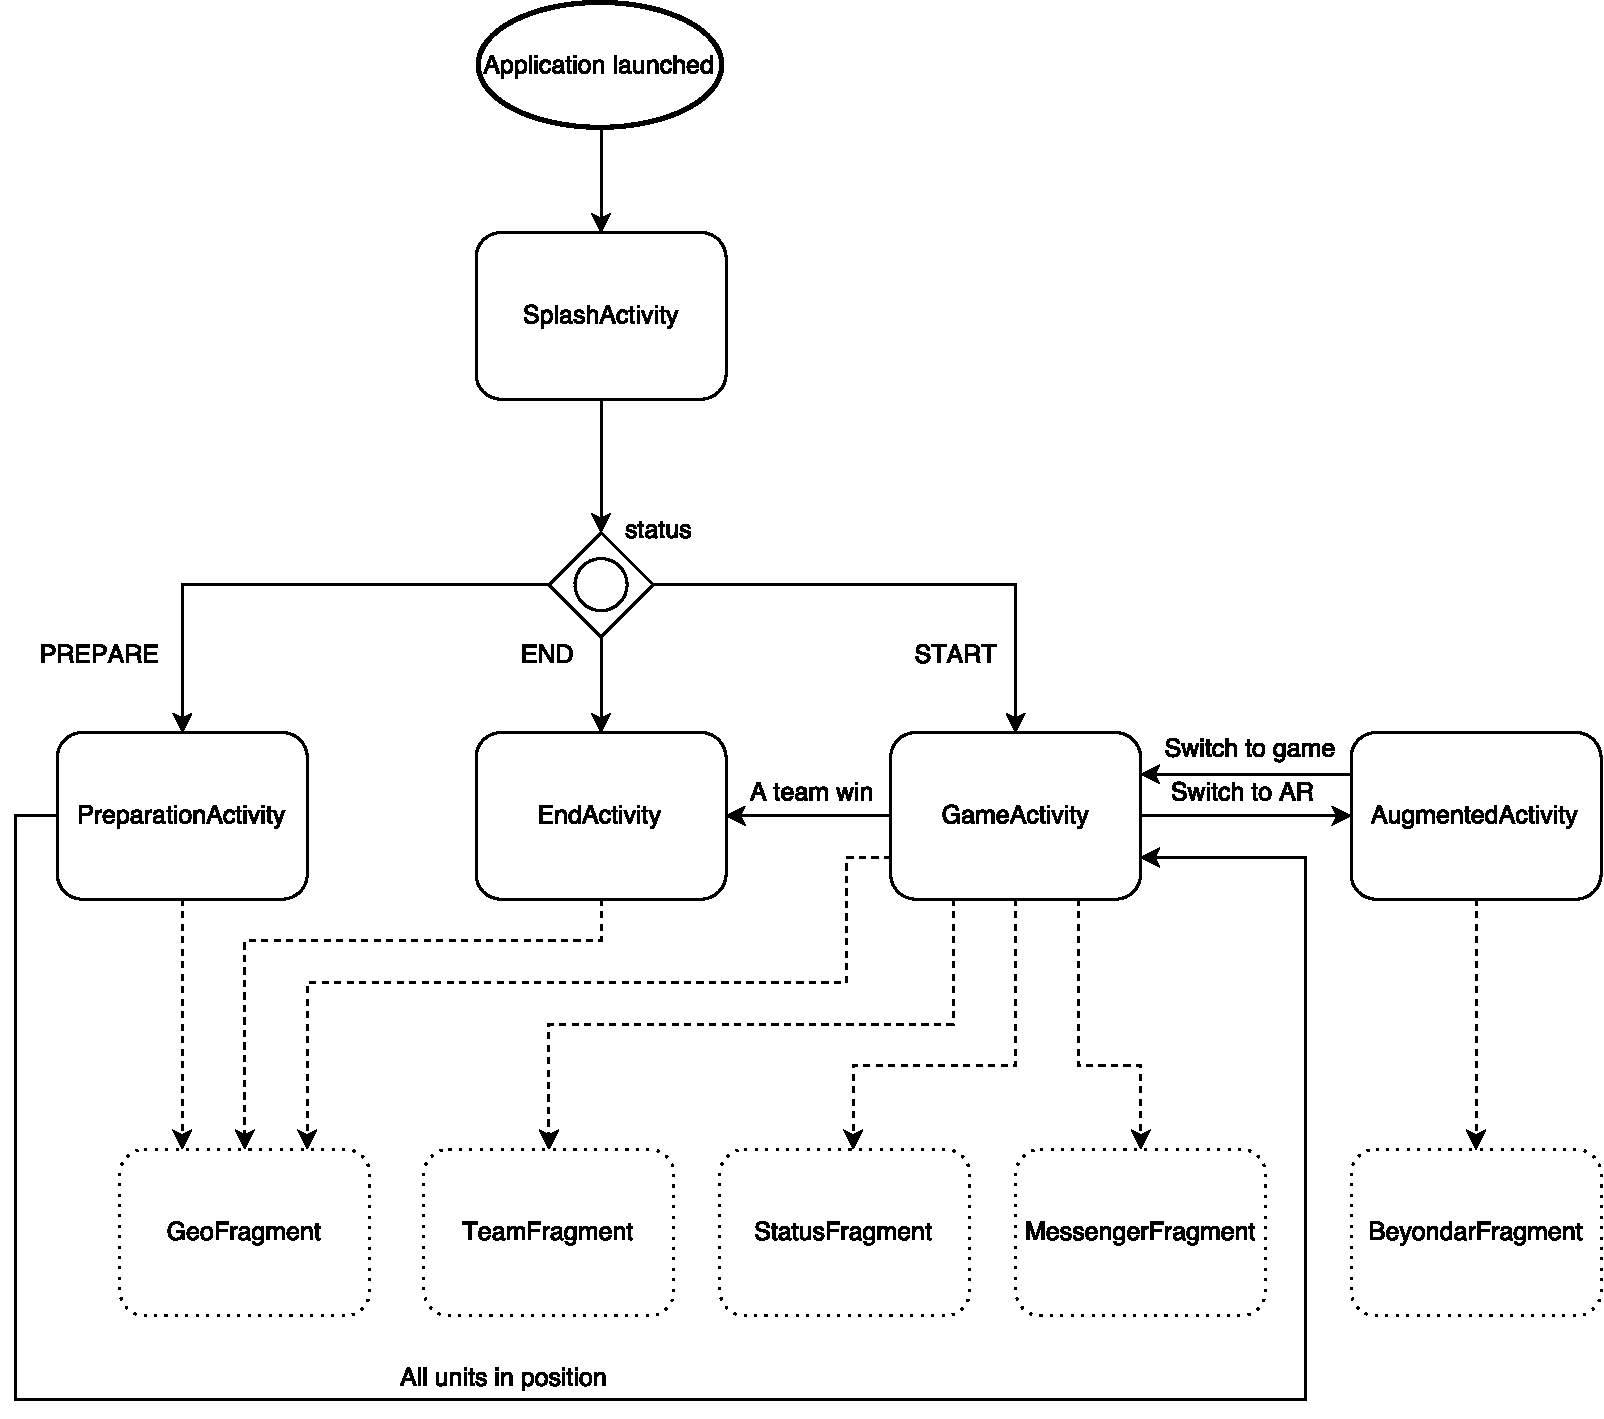
\includegraphics[width=\textwidth]{androidflowchart}
		
		\newpage
		
		Together with the game mechanics and rules description, a prototype of the game had been prepared for Android systems and it works from API 16 onward.
			
		Due to limited time and external job constraints, it has not been possible to finish the prototype in time for the graduation session, which is currently incomplete in some of its modules: messenger system has not been implemented, the augmented reality module which relies on the smart phone camera has not been properly connected to the prototype and with the action system, status fragment which should have shown information about other teams has not been implemented, the end game activity has not been implemented (from a practical point of view, it is more or less a copy of the preparation one).
		
		Following, a description of the features of every activity and fragment which composes the application.
		
		\paragraph{SplashActivity}
		
		It is composed by two alternative layouts: login and loading.
		Its main purpose is to perform the user login and pre-load all useful data for the following activity, which will be started after having understood in which status the game is in that moment.
		Everything it does is described in more details in \autoref{focus:splash}.
		
		\paragraph{PreparationActivity}
		
		It is composed by an instance of the \lstinline|GeoFragment| and its main purpose is to guide players to their starting point, forcing them to wait there that other units reach their as well. When everybody is in the right place, it starts \lstinline|GameActivity|.
		
		\paragraph{GameActivity}
			
		It is composed by a view pager (a group of tabs) which manages various aspects of the game.
		When a team successfully accomplish its objective, the game status is updated from the server and the application moves to the last activity of the game: \lstinline|EndActivity|.
		
			\subparagraph{GeoFragment}
			
			It is the most important fragment of the activity, because it lets you see the board, where other units are and data about the AR layer of the game.
			At code level, it is a wrapper around a \lstinline|MapFragment| (from Google Maps Android library) who takes care of managing the board and the zones of which it is composed, units position and the related visibility rules, AR objects which spawns around and many others tasks: its work flow is described later in \autoref{focus:map}.
			
			\subparagraph{TeamFragment}
			
			It is composed by four parts, each visible only during certain phases except the fourth one:
			\begin{description}
				\item[role management] displays the roles available during the \emph{ROLE} phase and lets the unit select its own;
				\item[action management] displays the actions available, related to the chosen role, during the \emph{ACTION} phase and lets the unit select its own;
				\item[money management] shows how many coins are present in the team reserve and lets unit borrow some of them in the \emph{MONEY} phase;
				\item[team mates status] it is a list showing the role, action and borrowed money of every unit in the team, it is visible in all phases of the game.
			\end{description}
			
			With these components, the activity manages three out of four phases by which the game is composed.
			
			\subparagraph{StatusFragment}
			
			It is composed by a general status bar, which shows some important data about the game (current turn, how many and which random events are left, etc.), and a list of team summary cards, one for each team playing (number of controlled zones, total money in their reserve, etc.).
			
			\subparagraph{MessengerFragment}
			
			It is similar to any other messenger system (Whatsapp, Allo, Facebook Messenger) and is implemented using the Firebase Cloud Messaging, not needing all the more advanced features (e.g., photos and videos).
		
		\paragraph{AugmentedActivity}
		
		It is a \lstinline|FrameLayout| containing a \lstinline|BeyondarFragmentSupport|, a wrapper of a normal fragment enhanced to display the camera captures as background, and an AR overlay which displays things based on the position of various objects and units.
		Its duty is to allow interaction among units and between them and AR objects, its behaviour is better described in \autoref{focus:augmented}.
		
		\paragraph{EndActivity}
	
		It is the last activity of the game and is composed by an instance of the GeoFragment as in \lstinline|PreparationActivity|.
		Its main purpose is to gather players to the end position, where the winner will be awarded. When everybody has reached it, the game finishes and the application force a logout of all players, changing the game status to \emph{INACTIVE}.
	
	\section{Main technological issues}\label{focus:general}
		
		While working on the project, some particular or complex problems required a not trivial solution, which resulted in some interesting pieces of code.
		Hopefully, the explanation about how they were solved here will be helpful for someone who will need to follow this same path in the future.
		
		\subsection{Board generation}\label{focus:board}
		
			While translating the rules from \textbf{Discworld - Ankh-Morpork} to the mobile game, the definition about how the board should have been, as seen in \autoref{design:board}, took some time.
			
			The initial idea was to obtain a randomly generated, asymmetric board contained in an irregular polygon defined by the event organizers.
			In this way, the playing ground could have been set to fit into different real-world city-related shapes (in Reggio Emilia case, the irregular hexagon made by the beltway was the most obvious shape to use).
			In addition, a randomly generated board would have prevented teams to study strategies based on a fixed map and would have forced them to improvise a new strategy while studying the map in \emph{PREPARE}.
			
			Unluckily, this kind of board generation almost immediately looked too advanced to be realized in a short time; in its place it had been deployed a more simple regular shape automatically derived from specified centre and radius.
			
			The simplest regular polygon that could be used was of course a circle, and that was the first choice until Google Maps polygons management got in the way. Circular shape was perfect for the board perimeter by himself, but zones perimeter where also needed for others in-game mechanics (checking in which zone each unit is, managing zone crossing, random point generation inside a given zone, etc.) and this was impossible to archive using the build-in circular shape of Maps API.
			The second thought was to replicate the external circular shape with polygons formed by many points, but that would have leaded to possible performance issues, given the number of points needed.
			In the end, as seen in the board image in \autoref{design:board}, a particular shape had been chosen in which the central zone is composed by 8 sides (one vertex every 45 degrees), four more zones are contained between the first zone perimeter and a ring composed by 16 sides (one vertex every 22.5 degrees) and last 4 zones are contained between the first ring and a second ring composed by 24 sides (one every 15 degrees).
			Zones between the second ring and the first one are shifted by 45 degrees because every zone must touch at least other 4.
			
			The fastest way to obtain all zones vertices, possibly also the simplest way apart from hard-coding their GPS positions, is to directly calculate the perimeter of every ring (the two mentioned earlier plus the central zone perimeter), putting all vertices in a multidimensional and ordered array representing zones perimeters.
			This is possible because zones are all adjacent, which means that many vertices are in common with multiple zones and it is enough to put them in the right order.
			
			At code level, this is achieved with three \lstinline|for| loops pretty similar one to the other, which seems to suggest that the procedure could be optimized even further by using polar coordinates, but the code is already complex as it is and for now the result is acceptable.
			The first and last loops calculate vertices clockwise, while the middle loop does it anti-clockwise; this is done because having alternately spinning loops makes much simpler to save vertices of all zones already ordered and get a closed shape for the polygons, as seen in \autoref{board:alternate}.
			
			\begin{figure}[htp]
				\centering
				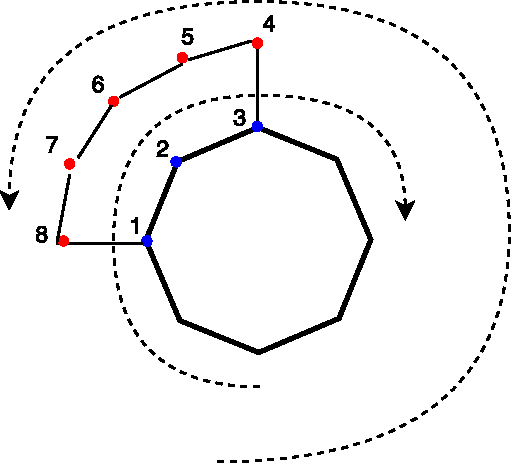
\includegraphics[width=.5\textwidth]{boardrounds}
				\caption{Graphical representation of alternate vertex calculation, showing the perimeter of one of the zones of the first ring}\label{board:alternate}
			\end{figure}
			
			Inside these loops, all points are obtained by starting from the board centre and calculating the new point based on the radius of the given ring and the offset angle which change at every iteration.
			
			It has to be noted that the board perimeter is not saved anywhere: only zones polygon are stored and printed upon the Google Map, for various reasons.
			First of all, single zones polygons on the map must be saved to be able to notice click events for some in-game mechanics: getting zone data, like which teams owns its power-up, or how many other units are present in the zone.
			Secondarily, the only feature which requires the board perimeter is the check about someone exiting it, but we can achieve the same result by checking if a position is inside any of the zones which had been saved: if it is not, the unit exited the board.
			
			\newpage
			
			\lstinputlisting[caption={Utility method, get new GPS position from given point, distance (ring radius) and angle}, firstline=158, lastline=171]{main/listings/boardfactory.java}
			
			\begin{figure}[htp]
				\centering
				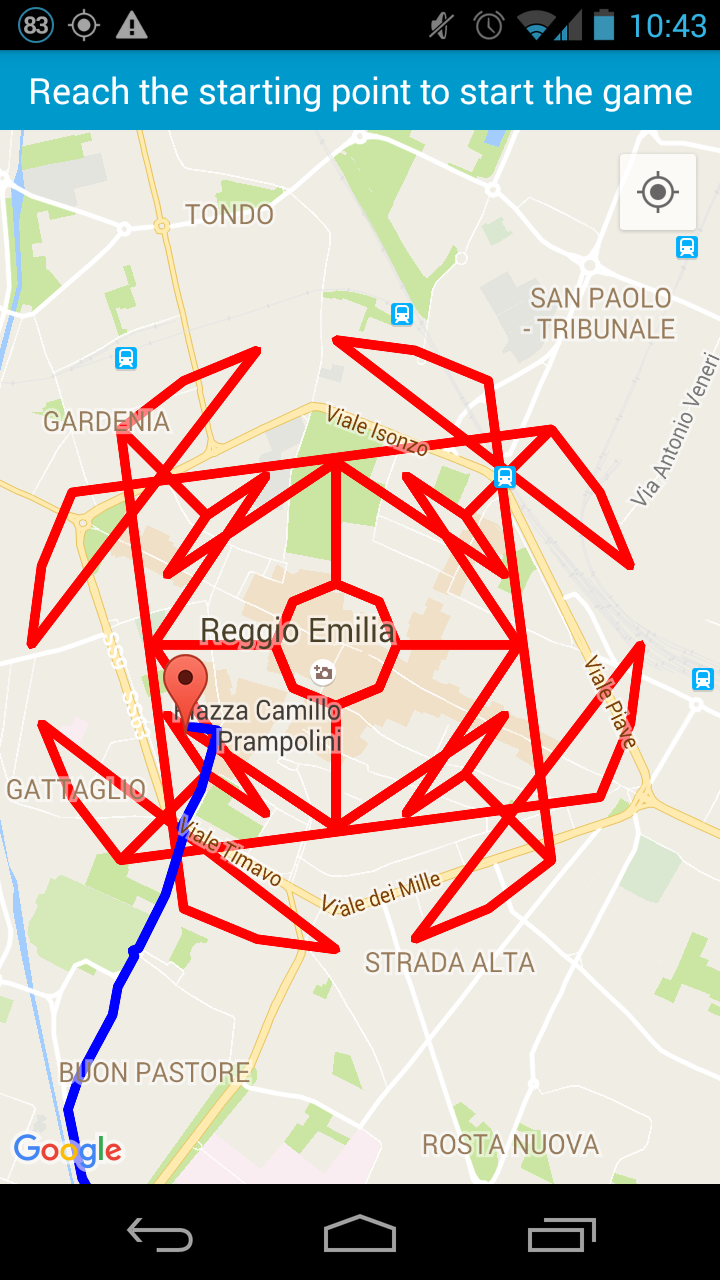
\includegraphics[width=.3\textwidth]{wrongboard1}
				\hfill % Stretches the space between images to align them to borders
				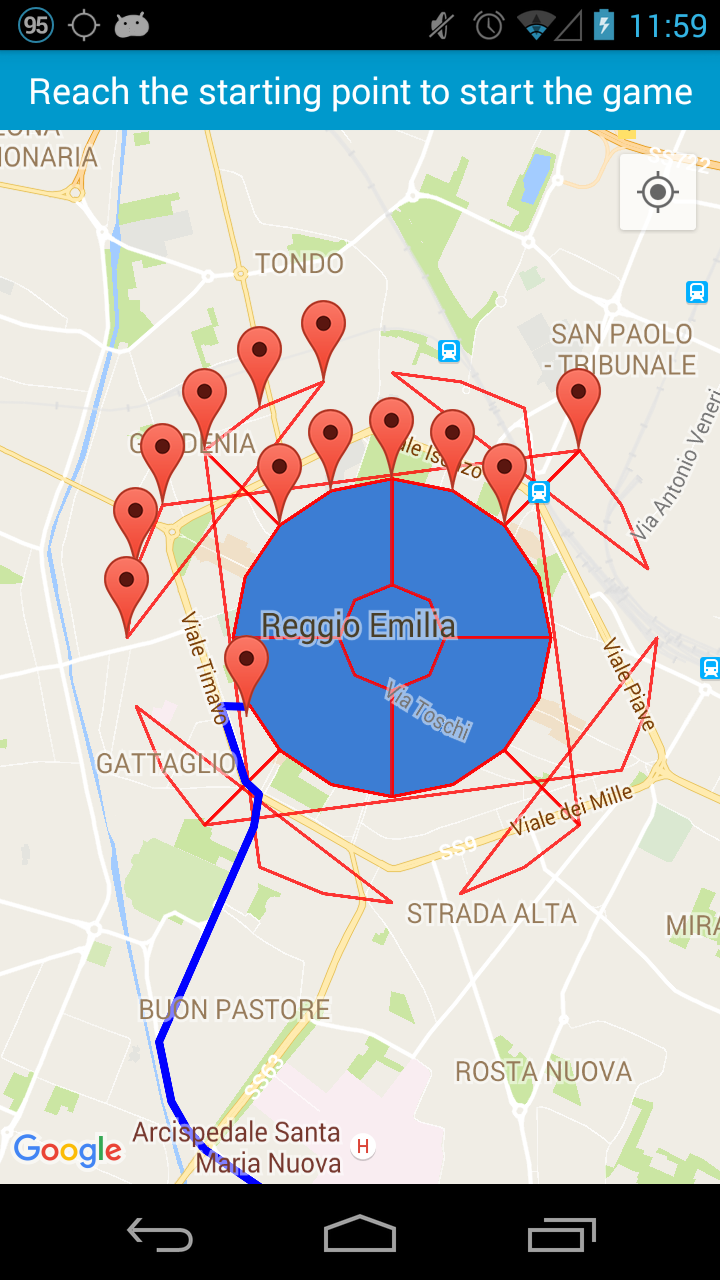
\includegraphics[width=.3\textwidth]{wrongboard2}
				\hfill
				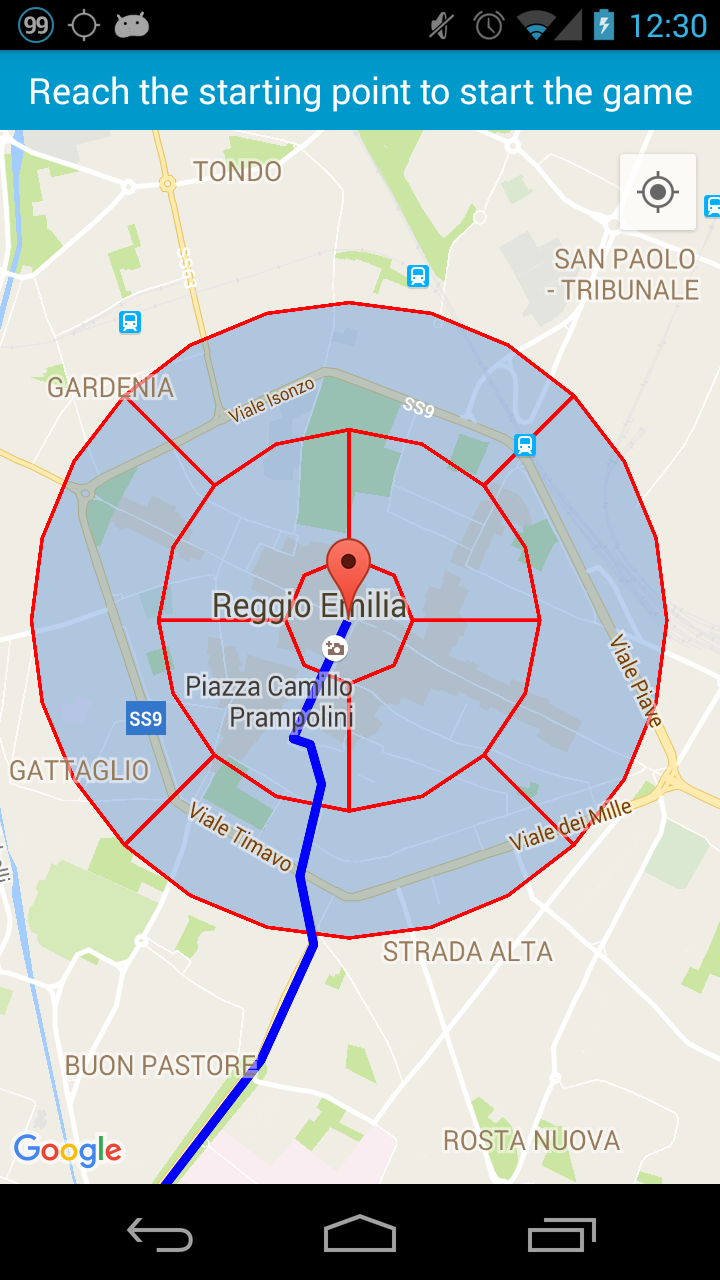
\includegraphics[width=.3\textwidth]{wrongboard3}
				
				\caption{Three board drawings trials while developing \lstinline|BoardFactory|}\label{board:mess}
			\end{figure}
			
			After some trial and error (\autoref{board:mess}), the right shape had been obtained, but the radius used to calculate the rings was obviously wrong.
			Considering that zones must have the same area, an R script had been used to find out which radius every ring should have had. Obviously the R script assumed the rings as circles, not as the weird shapes they actually are.
			
			After loops finish their run, the multidimensional array is used to fill in the perimeter \lstinline|ArrayList| of every zone on the board.
			
			The last part of the board fabrication is to make all zones aware of their neighbours. Unluckily, here hard-coding seems the only viable way, and for now the map is simple enough to allow for this.
			
		\subsection{Timer mechanism}\label{focus:timer}
		
			Synchronizing phases between server and clients is pretty easy with Firebase: taken that the server manages phase timers by its own without crashing and updates the phase field on game branch accordingly, devices just need to set a listener on it to know in which phase the game is.
			The task become less trivial when you add the constraint that all devices must have a synchronized countdown of the current phase.
			
			The first idea was to store, together with the current phase, also the timer duration.
			In this way, every device connected could just set an internal timer, nearly synchronized with the one on the server and the problem was solved.
			
			But let's go further: what if the devices must be able to connect/disconnect at will and still have the synchronized countdown feature?
			The must obvious idea would have been to add another field, perhaps the moment in which the timer started, together with its duration.
			
			To spare a field (which, in Firebase, usually means sparing an asynchronous callback and many troubles), the solution was to store, instead of starting time and duration, directly the expiration moment of the timer.
			For this to work, the time on every device and on the server must be the same. This is usually automatically managed by the operating system which uses internet to synchronize himself to the right time and can be took as assured on the server machine, but on players smart phones internal time could be modified by the users, which open the gates to possible glitches and cheats.
			
			Luckily Firebase comes to assist us on this as well: listening to the particular path \lstinline|.info|, a number of miscellaneous and useful piece of data can be accessed, one of them being the time offset between the local device and the Firebase server local time.
			
			Listening to \lstinline|.info/serverTimeOffset| value changes allow us to detect the current offset from the server, store it and add it to the countdown timer that displays the remaining time at every timer field change or device connection.
			
			To prevent every possible exploit, every time the timer field is changed on Firebase by the server, the local timer on every device is cancelled (if it was not expired yet), its \lstinline|onFinish| callback executed and the new timer is set up.
		
		\subsection{Match logging}\label{focus:log}
		
			To better study the game mechanics effectiveness a replay feature may be useful and could be used also to detect cheaters or problems.
			
			For this, a logging system had been prepared, which keeps track of all units' actions, as well as their movements, and various in-game events.
			
			The \lstinline|GameLogger| class is a singleton that statically provides a logger which writes to a file in the \lstinline|/log| path, appending the creation time stamp to the log file name to log multiple game sessions.
			
			All server model classes implements the \lstinline|FirebaseSync| interface, which ask to override the \lstinline|sync()| method.
			In this method, called at the end of the constructor, all listeners to useful data from Firebase must be set.
			In this way, all instances will auto-update themselves, listening for changes on Firebase, and while doing so they will also log all the meaningful actions and events which will be taking place during the match.
			
			When the game finishes, the structured log file could be set as input of an ad-hoc decoder, reproducing the events like a video.
			
			This ad-hoc decoder has not been developed yet, but it is easy to implement. 
		
		\newpage
		
		\subsection{Random picker}\label{focus:picker}
		
			\lstinputlisting[caption=Random picker class]
							{main/listings/randompicker.java}
			
			A small but useful function which is missing from Java \lstinline|List| interface implementations is the possibility to extract a random object from a given list.
			This seems useless, but nearly all games need some random extractions and in particular contexts (e.g., testing purposes) a small feature like this can come handy.
			
			In this project, randomly assigned values are used in many parts, e.g., objectives distribution to teams, and many parts not yet completed will heavily rely on random generation and extraction.
			
			For these reasons, a small utility class had been written to extract random values from a given list. It exposes two methods:
			\begin{description}
				\item[pick] takes the random seed of this thread, then randomly picks an integer value between 0 and the list size -1 and returns the list element associated to that value. 
				\item[extract] same as \lstinline|pick| method, but removes the extracted object from the list before returning it.
			\end{description}
		
			The picker uses \lstinline|ThreadLocalRandom| class instead of the more known \lstinline|Random| because, relying on asynchronous callbacks and on multi-threading, the synchronized access overhead to the process-global class may decrease performance.
			Plus, it is the recommended class to use, as written in Java 8 documentation.
						
		\subsection{Random point generation}\label{focus:point}
			
			A method to generate random points is needed to implement most of the AR interactions; those points must usually be inside a given zone perimeter.
			
			Generating coins inside every zone for the collectors, drawing a path composed by random points to calm a zone or make it chaotic and other actions, rely on this function.
			
			On Android, it is easy to get the previously saved Polygon of a zone and generate a point within its bounds, checking later if the point is actually inside its shape\footnote{Let's remember that a Polygon shape and its bounds are not the same thing: the shape can be irregular, while its bounds are the smallest rectangle around the shape which contains all its points} with Google Maps PolyUtils support library, but on the server we do not have such a powerful tool.
			
			The \lstinline|RandomPoint| class had been written to address this deficiency.
			
			Given as input a generic perimeter (this can also be the board itself or an area around a given player), the method will generate a \lstinline|Path2D| region from it, giving access to the \lstinline|Path2D.contains(x,y)| method.
			
			Then it will get the region bounds and keep selecting a random point inside that rectangle until that point is also contained inside the given region.
			
			Once an acceptable point is found, it is returned wrapped in a \lstinline|GeoLocation| object.
			
			\lstinputlisting[caption=Random point generator class]
			{main/listings/randompoint.java}
		
		\subsection{Zone control manager}\label{focus:control}
		
			The \lstinline|ControlObjective| needs a special mechanics to understand which team currently controls a given zone.
			A zone is controlled by a team if the sum of its buildings and units there is greater than the one of every other team.
			If two or more teams have equal sum, nobody controls the zone.
			In the Firebase data model, the controller team is specified in the \lstinline|controller| field, which is updated by the server.
			In fact, every time a unit changes zone or a building is constructed/demolished the server replicates that information on the selected zone instance using the \lstinline|addUnit|, \lstinline|removeUnit|, \lstinline|addBuilding| and \lstinline|removeBuilding| methods.
			Every one of those, after updating their own \lstinline|ArrayList| of units/buildings, calls \lstinline|updateController|.
			This method, which ask for a team reference and an integer as arguments, updates the control \lstinline|HashMap| which keeps track of the sum of buildings and units of every team, then search the entry where that value is the maximum.
			Every time a new maximum is found, its team reference (which is the key of the \lstinline|HashMap| entry) is stored as the controller team, but if a second entry with the same value is found, the controller team reference is set to null.
			After cycling all the entries, the controller variable is set to the right team reference (or null if no one controls the zone) and it is accessible with \lstinline|getController| method.
		
		\subsection{Presence system}\label{focus:presence}

			It is important, both for team mates and enemies to be able to see if a given player in their zone is currently active (e.g., he is using the application, his GPS position is accurate) or not.
			
			Using Firebase, setting up a presence system is trivial, thanks to official guides\cite{firebase:presence} and ad-hoc tools provided by the library.
			
			The \lstinline|OnDisconnect| object can be chained with the \lstinline|Query| one to store a particular operation on the server, which will be executed when the connection with the client interrupts.
			
			The presence system is required in four different activities and thus it had been put in a singleton class, \lstinline|PresenceManager|, which exposes two static methods: \lstinline|PresenceManager.setup(userId)| and \lstinline|PresenceManager.cancel()|.
		 
			\paragraph{setup}
			This method initializes the presence manager using the given user id.
			If the singleton had already been initialized, the user id is checked against the previously saved one: if it is the same, no operation is done and the presence manager is shared between different activities saving some overhead, otherwise the \lstinline|cancel| method is called and a normal set-up takes place.
			If instead it is the first initialization, the user id and some disconnection listener references are stored internally, then a value listener on the particular location \lstinline|.info/connected| is added: like many values stored on the special \lstinline|.info| branch, this field is updated directly by Firebase, in this case upon client's connection state changes.
			As soon as the \lstinline|.info/connected| callback is fired with value \lstinline|true|, a new branch with the user id as key is pushed into the \lstinline|presence| branch (see \autoref{model:presence}) and two operations are stored on the server to be executed upon disconnect event: the first one removes the value from \lstinline|presence| branch, while the second updates \lstinline|lastOnline| field inside the user personal branch.
			In this way, it is easy to check which users are currently connected reading \lstinline|presence| branch children, and it is easy as well checking the last moment in which a particular user disconnected.
			
			\paragraph{cancel}
			If the singleton has actually been initialized, this method resets the presence manager removing all values and disconnect listeners.
		
		\subsection{Splash screen and data pre-loading}\label{focus:splash}
		
			To avoid long loading times once inside the application, most of the common data to all activities are retrieved in the splash activity, which also manages players login.
			These data are stored into the shared preferences or sent as extras attached to intents.
			
			The splash screen is composed by two alternatively shown layouts: login and loading.
			Login layout shows the application icon, email field, password field and login button.
			Loading layout instead is not interactive and shows a loading animation and a textual component which inform the user about which operations are being performed.
			
			Numerous steps must be executed before the application can start flawlessly:
			\begin{itemize}
				\item perform login or auto-login;
				\item retrieve unit and team id;
				\item enable GPS;
				\item retrieve current location;
				\item check game current status.
			\end{itemize}
			
			\paragraph{Login}
			By default, the loading layout is the visible one, considering that thanks to an auto-login feature the login layout is visible only for the first access or if an error occurs.
			The email and password are stored in shared preferences after the first login and automatically inserted into the appropriate fields in the subsequent accesses: if both email and password are actually present, the auto-login feature is turned on.
			
			When auto-login is not enabled, login layout is shown in place of the loading one and the user is prompted to insert his credentials, which will be then used to initialize a Firebase Auth session.
			
			Firebase Auth natively provides a token-based auto-login feature, but its implementation is buggy; after the Firebase Auth system initialization, its attempt to perform it is blocked and, if needed, the home-made one is activated.
			
			The auto-login home-made implementation uses previously saved credentials (losing some security with respect to the token-based system), to simply perform a normal login procedure, but automatized by the code.
			
			After the user logged in successfully, his \lstinline|lastOnline| field is updated.
			
			\paragraph{Unit and Team ids}
			
			Unit id and team id are crucial for all activities: they are used in \lstinline|GeoFragment| (used in \lstinline|PreparationActivity|, \lstinline|GameActivity| and \lstinline|EndActivity|), \lstinline|TeamFragment|, \lstinline|AugmentedActivity|, etc. Those are almost \emph{all} the important parts of the application.
			If every component had to retrieve them by its own (as it was at an earlier stage of the project), the code would have been a mess, with duplicate code in every class performing a call to the Firebase Auth system to get the user id and then to Firebase Database to get the team id using the previously retrieved user id.
			For this reason, those ids are directly retrieved right after the login and stored in the shared preferences to be accessible in every activity of the application.
			
			When performing the login, user id comes for free: during unit branch creation, its id is set as the same from Firebase Auth system, so it can be retrieved using \lstinline|FirebaseAuth.getCurrentUser().getUid()|.
			Team id is retrieved right after, using a specific Firebase Database request upon the unit branch.
			
			\paragraph{GPS}
			
			Being a location-based AR, the GPS service must always be enabled while using the application, so the first thing to do is to switch it on.
			To do so, \lstinline|GoogleApiClient| must be initialized first and the system location service can then be retrieved.
			If its GPS provider is already enabled (which means, if the GPS feature is turned on), this step can be skipped, otherwise the provider must be activated: a new dummy \lstinline|LocationRequest| is created and launched, thanks to the previously initialized \lstinline|GoogleApiClient|, to check if it can be activated.
			If the request says the GPS can be enabled,  \lstinline|startResolutionForResult| method provided by the GMS API is used to ask the user the permission to enable it on his behalf, otherwise there is a problem with the GPS provider which cannot be resolved: the error is notified to the user and the login layout displayed.
			If the user declines the request of turning on the GPS, an error is displayed and he is kindly asked again to do so, until he accepts.
			
			\paragraph{Current location}
			
			Having obtained GPS permission, \lstinline|FusedLocationApi| is used to get the last known location of the device with \lstinline|getLastLocation| method.
			This powerful tool gets all location service providers available in that moment (cellular network, Wi-Fi, GPS, smart phone sensors) and mix their data to get the most accurate position obtainable, exposing a simple API which can let the developer define which retrieve mode must be used (low battery consumption, high accuracy, etc.) while reducing at its best battery drain.
			The last known location is kept by Android system, which saves the value of the last position retrieved by any application or service using Google Play Services on that device.
			Having retrieved a more or less accurate unit's current position, it is stored and the last step of the initialization procedure is performed.
			If there is no last known location (\lstinline|getLastLocation| returns a null pointer), a \lstinline|LocationRequest| is set up and launched to retrieve it.
			
			\paragraph{Game status}
			
			Considering that the game can have any status when the user accesses the application, the last step is to query Firebase Database to check the current status and start the next activity accordingly.
			\begin{itemize}
				\item \textbf{\emph{INACTIVE} or \emph{INITIALIZE}:} the user is noticed that the game cannot be accessed yet;
				\item \textbf{\emph{PREPARE}:} \lstinline|PreparationActivity| is started, which helps the players to displace correctly on the game board;
				\item \textbf{\emph{START}:} \lstinline|GameActivity| is started, which manages the entire game;
				\item \textbf{\emph{END}:} \lstinline|EndActivity| is started, which informs all players of who won the game and gathers them to a common place where the winning team will be awarded and the event will continue.
			\end{itemize}
		
		\subsection{Navigation drawer template}\label{focus:drawer}
		
			Even if the final version of the application does not include a navigation drawer, the absence of a simple yet flexible implementation of it, which could be applied smoothly to multiple activities, is puzzling.
			Moreover, the project needed a template to avoid rewriting the common frame of all activities (coordinator layout and its behaviour, action bar, information bar).
			Given this, an implementation of it had been realized.
			
			All findable guides about this topic are based upon defining every single activity as implementing the navigation drawer interface.
			A more advanced idea is to define an abstract class which extends the activity class and implements the navigation drawer interface, making all activities extend it.
			In this scenario, the activity must call an initializer function in its \lstinline|onCreate| method, which could lead to oversights and errors difficult to track down. Moreover, the \lstinline|setContentView| is still delegated to the activity, meaning that its XML layout code is still product of the copy/paste of all navigation drawer views between an activity's layout file and the other.
			
			The developed solution is still sort-of based on this idea, but is more general: the \lstinline|NavActivity| abstract class load an XML layout with the navigation drawer feature, which in turn include a second XML layout with all other frame components.
			This division let the developer see in Android Studio preview how the frame graphics will be both with the open navigation drawer and the closed one.
			\lstinline|NavActivity| takes care of the common operations to every activity, mostly initialization and management of action bar, information bar and navigation drawer.
			The XML template layout is a \lstinline|CoordinatorLayout| whose children are an \lstinline|AppBarLayout|, a \lstinline|FrameLayout| and a toolbar which acts as information bar.
			The \lstinline|FrameLayout| is a place-holder, it is set as content view and sub-sequentially the specific activity layout is inflated inside it.
			
			To know which layout we have to inflate into the template, an abstract method called \lstinline|getContentLayoutId| is defined.
			All activities extending \lstinline|NavActivity| are forced to implement this method which must return the id of the layout to be inflated, this avoid possible oversights.
			
			This system also reduce code redundancy and copy/paste actions to zero, removing one of the major error generator while coding.
		
		\subsection{AR on map}\label{focus:map}
		
			One of the most complex yet fundamental challenge which had been faced, was the definition and creation of the \lstinline|GeoFragment|: a class wrapping the \lstinline|MapFragment| from Google Maps API and over which half of the application AR layer had been built.
			
			The main problems bound to this component were the continuous retrieving of the user position, other players tracking and displaying, and the implementation of the visibility rules among users or between users and AR objects.
			
			Additionally, as described in \autoref{app:workflow}, this component is used in three different activities: \lstinline|PreparationActivity|, \lstinline|GameActivity| and \lstinline|EndActivity|.
			The problems are the same for all activities, but must be managed differently based on which activity is instantiating the fragment.
			
			Other tasks performed by this component, either trivial or already discussed in other parts of this document, are: map customization, zones download and board drawing, team color download and markers pre-loading.
			
			\newpage
			
			\subsubsection{Location sniffer}
			
			\lstinline|MapFragment| by its own already comes with an easy to activate and use \emph{My Location} layer, which saves us some trouble while adding some others.
			In fact, the default \lstinline|LocationSource| used for that layer is an internal one from which is not possible to get the location updates from an external piece of code: once it is set up, the location updates are directly sent to the \emph{My Location} layer.
			This meant that either the entire layer should have been recreated or two location service requests had to be activated. They were both unpleasant options, a more graceful third one had been searched, and found, which consist in a new utility component which implements the \lstinline|LocationSource| and \lstinline|LocationListener| interfaces and replicates the Google internal \lstinline|LocationSource| implementation as best as possible; this component, called \lstinline|LocationSnifferSource|, takes as parameters the activity to which is bound and an object implementing the \lstinline|LocationSniffer| interface (usually the activity itself) and sends every location retrieved to the sniffer class right after sending it to the rightful object that activated the location source (in this case, the Google \emph{My Location} layer).
			
			In this way we are piggybacking on the location which would have been retrieved anyway by the \emph{My Location} layer avoiding asking for a location twice every time or to re-implement that layer.
			
			This component is then set as the \lstinline|LocationSource| which must be used by the Google Map component; this also prevent leaks, because the location source will be activated and deactivated automatically by the Google Map upon \lstinline|onStart|/\lstinline|onStop| methods of the \lstinline|MapFragment| life-cycle.
			
			\subsubsection{Other players tracking and displaying}
			
			Considering that every unit in game \emph{could} be visible over the board at any time and that the visibility rules change as the game phase or status do so, players are tracked storing all theirs data but activating a listener on their position only when they must really be shown on the board.
			
				\paragraph{Unit model}
					
				To keep the data of the units related to their representation on the map, a private class had been created: \lstinline|UnitData|.
				This class holds unit general information (id, team, role) together with some data related to its location (GPS position and current zone), a reference to its marker and a location listener one.
				
				Role and current zone are automatically updated when they change on the database, this automatic sync is vital to the visibility system.
				
				The location field represent the last known GPS position of the unit, while the location listener reference is added or removed depending on if the unit must be visible or not (we do not need to keep track of the movements of units we cannot see).
				
				The marker reference is used when the unit last known location is updated, causing the marker itself to move on the board or, when a unit disconnects, causing it to become partially transparent.
			
				\paragraph{Unit initialization}
				
				During the first setup of the fragment, an \lstinline|HashMap<String,UnitData>| is filled with an entry per unit in game.
				This entry is filled with the id, the team and the current role of the unit, referenced by its same id.
				The unit is initially assumed to be out of the board, so we set the zone equal to 0: a listener is then added to keep the zone value synchronized with the database.
				We set the current position to a dummy \lstinline|LatLng| in (0,0). This is needed because we are not sure that the unit currently have a position set on the database, but we \emph{must} provide one where to place the marker on the board.
				The marker icon is a circular dot with the color of the team of the unit, its title is the unit user name and by default is set as not visible.
				
				A listener is added to keep the unit role in sync with the database, while another one keeps track of the presence of the unit (changing the transparency of the marker accordingly).
				
				Units which are in the same team as the current user are automatically set as always visible, and their location listener is activated.
				
			
			\subsubsection{Visibility rules} \label{focus:map:visibility}
		
			Obtaining a clean code while managing the visibility rules had been a hard task, and several structure rethinks were needed before finding an acceptable solution.
			This would have been trivial if all units could just see everybody else, but the idea was to limit their sight to force collaboration and communication among team mates and to push them into trying to foresee other team movements from incomplete data.
			This is why the visibility rules change accordingly to the game phase: while in \emph{TURN} phase the sight is limited and they must make assumption on what other teams are doing, in any other phase all units are visible, in this way the players can check if their assumption were right and can access the whole picture for some time to continue this prediction mind game.
			
			\begin{table}
				\caption{Visibility rules}
				\label{focus:map:visibility:rules}
				\centering
				\begin{tabular}{lcccc}
					\toprule
					\multirow{2}*{Game status} & \multicolumn{4}{c}{Current user role} \\
					\cmidrule(lr){2-5}
					& \emph{COP} & \emph{ASSASSIN} & \emph{BUILDER} & \emph{COLLECTOR} \\
					\midrule
					\emph{PREPARE} or \emph{END} & \multicolumn{4}{c}{Everyone, in all zones} \\
					\emph{START} not in \emph{TURN} phase & \multicolumn{4}{c}{Everyone, in all zones} \\
					\emph{START} in \emph{TURN} phase & \emph{ASSASSIN} & \emph{BUILDER} & Everyone & No one \\
					\bottomrule
				\end{tabular}
			\end{table}
			
			The visibility rules are summarized in \autoref{focus:map:visibility:rules}: while the most are just a matter of enabling/disabling location listener of all the units and show/hide the respective markers, the most interesting to analyse are the ones of \emph{TURN} phase, which are applied in two steps. 
				
				\paragraph{Zone limitation}
				
				The user sees only the units in his own zone (except from his team mates which are always visible). Initially, this had been done setting a listener on the zone field of every unit and checking if they were in the same one as the current user, but it proved to be an infeasible solution given the growing complexity of managing consistently many listeners related to a vital aspect of the application.
				The current solution is based on the fact that every player, upon his device GPS position change, updates his current location and checks by his own in which zone he is in, updating that piece of information as well.
				While doing so, the user now updates also the list of units present in a zone, both for the zone he is entering, adding himself in, and for the one he is exiting, removing himself from it.
				Listening to that users list of the zones automatically informs the current user of which marker he can show, provided that the listener changes the target zone accordingly to his movements.
				To avoid possible “flickering” when a user is on the border of a zone, a delta value is added to the check (10 meters) and must be surpassed to actually change the active zone.
				
				\paragraph{Role limitation}
				
				The user sees only some kind of other units, as shown in \autoref{focus:map:visibility:rules}.
				This is accomplished with a rule \lstinline|HashMap<Role,Role>| which, given as key the current user role, select which role must have the other units to be visible.
				This is a limitation but also a useful information: if you are a cop, you know that all the enemy units you are seeing in the zone are assassins, for example, and act accordingly to protect your team mates.
				
		\newpage
				
		\subsection{AR on camera}\label{focus:augmented}
			
		While the map is all a matter of \emph{seeing} AR objects and other units, the actual interaction with the augmented world take place in \lstinline|AugmentedActivity|.
		This activity is composed by a \lstinline|BeyondarSupportFragment|, which by its own is a \lstinline|GLSurfaceView| with transparent background, where AR objects are rendered, placed in front of a common \lstinline|SurfaceView|, where the frames caught by the camera are redirected. In this way we can see the AR objects placed in the real world, based on their GPS position and other device sensors.
		
		This activity is accessible via the \lstinline|GameActivity|, and a button is displayed to take the user back there when he is done using the AR module.
		It is important to note that this activity is accessible only during the \emph{TURN} phase while the game is in \emph{START} status: if the user is in this activity when the timer expires, it will be automatically redirected on the \lstinline|GameActivity|.
		
		While the concept of zone is less relevant in this mode, because the visibility rules does not involve them, a simplified version of the system used in \lstinline|GeoFragment| is re-used here as well, to keep data on Firebase up to date.
		
		The phase timer, more useful than ever in this mode, is retained from \lstinline|GameActivity| but displayed in a more discreet way.
		
		The work flow of this activity is pretty straightforward: when started, it requires the objects within a certain radius around the given initial location and use them to initialize a \lstinline|World| instance, an abstraction provided by the Beyondar framework.
		Then a location request is registered to keep the position of the player updated inside the \lstinline|World| representation, while other players and AR objects will be added/removed dynamically from it when they exit the given radius. In case the user tries to disable the GPS sensor, an error message is displayed, he is logged out and it will be asked to re-enable it.
		
		Two main problems had been faced for this component: other players tracking and displaying, and interactions with AR objects and units.
		
		\textbf{Due to time constraints, the second one has not been implemented, just designed.} 
			
			\subsubsection{Tracking and displaying}
			
			With respect to the map AR part, other players tracking is a lot easier, thanks to an add-on available for Firebase: GeoFire.
			This library allows us to perform geo-queries: query on the database which retrieves all pre-registered objects/players within a certain radius.
			The visibility rule for this component had been thought to be pretty straightforward, given that when using it players will be in the most dynamic moments of the turn phase and people will be probably running around: every player closer than 25 meters from the current user is displayed, with a label on his head which identifies his team and role, and every AR object closer than 80 meters is displayed as well.
			These rules are enforced by two geo-queries, considering the two different rays, which monitor all the entering and exiting players/AR objects and which criteria (the centre of the geo-query) is updated every time a new GPS position is retrieved by the device.
			
			Every unit trying to interact in any way with the AR world will be visible, because to access and use the \lstinline|AugmentedActivity| the GPS must be active and the location updates with it.
			The fact that \emph{all} interactions are possible only via this activity limits scenarios where, for example, assassins reach their prey with the application or GPS turned off to catch it by surprise.
			
			\subsubsection{Interactions}\label{focus:augmented:actions}
			
			Interactions via the augmented reality world can assume various forms, usually some kind of mini-game, and depends from the role and action chosen by the current user.
				
			{ % Creates a group to stretch this content in a single page
				\setstretch{0.87}
			
				\paragraph{Follow the path}
				It is the one used for the \emph{CALM} action of the \emph{COP} and the \emph{PANIC} action of the \emph{BUILDER}, which both alter the current zone chaotic status.
				It basically consists in following a path composed by multiple POIs inside the current zone. The points can be actual POIs taken from Google repositories or simply on-the-fly randomly generated points inside the zone by the application.
				An arrow will always point towards the next POI which must be reached, the distance to reach it will be displayed as well, and a graphical effect (depending on the setting of the game) is generated every time one is reached.
				
				\paragraph{Collect}
				It is the one used for the \emph{COLLECT} action of the \emph{COLLECTOR}, which can gain randomly generated coins for his team.
				This interaction resembles the previous one, except that the coins are AR objects shared between all players (once one is collected, it disappears from the display of all others collectors) and must be mined. The mining process can be a tap-hold or multiple taps, the important thing is that the collector must stay over the same coin at least 10 seconds: this creates a weak spot where assassins can recognize them and eventually take them down. The number of collectors already present in a zone is displayed, in case the current player prefers to move to a zone with fewer collectors, hoping to have less competition while gathering the coins.
				Another difference from the \textbf{follow the path} interaction is that there will be multiple arrows pointing to the three coins closer to the current player, instead of just one.
				
				\paragraph{Stay near here}
				It is the one used for the \emph{PROTECT} action of the \emph{COP} and the \emph{ASSASSINATE} action of the \emph{ASSASSIN}, both related to the assassination mechanism.
				The bases are the same for both actions: when within a certain range from another unit it is possible to mark it as the target of your action, then you have to get near that unit into a smaller range, if you manage to stay within this second range for a given amount of time, your action succeed, otherwise you fail and must repeat the procedure after a cool-down time.
				What differs between the two actions are the meanings and values of the various phases.
				
				
				For the cop, the first range is 10 meters, the second one is 4 meters, the time in which he can stay within 4 meters by his target is 15 seconds and for all that time the cop himself and the protected unit cannot be targeted by assassins (if the unit was already the target of an assassin, the assassination fails). The cool-down of this action is 10 seconds, after which you can re-use it (both in case of failure or success).
				This action is indeed pretty boring if compared to the others, but hopefully it will be mitigated by the fact that who takes it will be always together with at least one of his team mates.
				
				
				For the assassin, the first range is 5 meters, the second one is 3 meters, the time in which he must stay within 3 meters by his target is 4 seconds. If he manages to kill his target, he cannot perform other kills for that turn. If he fails, the cool-down time is 5 seconds, after which he can retry the assassination. He can repeat this until he succeeds or the \emph{TURN} phase timer expires.
				When the assassin select a target, his phone will emit a sound to alert him and, if he is using the application in that moment, the screen will reflect the danger situation.
				
				\paragraph{Perform gestures}
				It is the one used for the \emph{BUILD} action of the \emph{BUILDER} and the \emph{DEMOLISH} action of the \emph{ASSASSIN}, both related to the buildings' mechanism.
				This kind of interaction must keep who performs it occupied for 1 minute and half or more, giving the importance that these actions have on the game in many of its parts (power-ups management, the money usage, the control of a zone, etc.) and consist in a random flow of different gestures which must be executed by the player. If the gesture is executed correctly and with the right timing, it scores a point (or more points in case of combos), if it does mistakes, it loses a point. While this points pool increase, the building object is shown to grow/spoil, depending on the action, on the AR layer, and when it reaches a certain value (150 for example), the building is completed/destroyed and is added/removed from the database and map.
				Gestures can vary from simple touch and swipes to more advanced and particular once, like touch-less gestures and blow recognition offered by some SDKs\footnote{Snapback (http://www.snapback.io/), even if not yet publicly available, can be an interesting partner to add not standard gestures.}.
				Buildings can be constructed only within a radius of 30 meters from the zone centre.
				
			}